\section{16 January 2019}
\begin{defn}
Let $T: V\to W$ be a linear transformation. The range or image of $T$ is the is the set range $\mathscr{R}(T)=T(V)$=im(T).
\[\{\Vec{w}\in W\ |\ (\exists \Vec{v}\in V) \Vec{w}=T(\Vec{v})\}\]
\end{defn}
\begin{defn}
The kernel or nullspace of $T$ is $ker(T)=\mathscr{N}(T)$.
\[\{\Vec{v}\in V\ |\ T(V)=\Vec{0}_W\}\]
Note: The kernel is a vector space.
\end{defn}
\begin{center}
    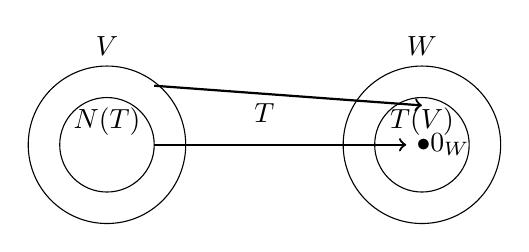
\begin{tikzpicture}
    \draw (1,0) ellipse (1cm and 1cm) node[above] {$\mathscr{N}(T)$};
    \draw (5,0) ellipse (1cm and 1cm);
    \draw (5,0) ellipse (0.6cm and 0.6cm) node[above] {$T(V)$};
    \draw (1,0) ellipse (0.6cm and 0.6cm);
    \draw (5,1.25) node {$W$};
    \draw (3,0.4) node {$T$};
    \draw (1,1.25) node {$V$};
    \draw[thick,->] (1.6,0) -- (4.8,0) node[right] {$\bullet\Vec{0}_W$};
    \draw[thick,->] (1.6,0.75)--(5.0,0.5);
    \end{tikzpicture}
\end{center}

\begin{bmatrix}
\end{bmatrix}
\begin{ex}
Let $T:\R^2\to\R^3;\ T(\begin{bmatrix}x\\y\end{bmatrix}) =
T(\begin{bmatrix}x+3y\\-x+y\\2x+y\end{bmatrix})$.
\[ker(T)=\{\begin{bmatrix}x\\y\end{bmatrix}\in \R^2\ |\ T(\begin{bmatrix}
x\\y\end{bmatrix})=\begin{bmatrix}
0\\0\\0
\end{bmatrix}\in \R^3\}\]
\[x+3y=0\]
\[-x+y=0\]
\[4y=0\implies y=0 \implies x=0\implies ker(T)=\{\begin{bmatrix}
0\\0
\end{bmatrix}\}\]
\[T(V)=\{\begin{bmatrix}
x+3y\\-x+y\\2x+y
\end{bmatrix}\ |\ x,y \in \R\}\]
\[T(V)=\{x\begin{bmatrix}
1\\-1\\2
\end{bmatrix}+y\begin{bmatrix}
3\\1\\1
\end{bmatrix}\ |\ x,y\in \R\}=\{t\Vec{a}+s\Vec{b}\ |\ t,s\in\R\}\]
Which plane is it? Contrast $L(\begin{bmatrix}
x\\y
\end{bmatrix})=\begin{bmatrix}
x\\y\\0
\end{bmatrix}$.\\
%\begin{center}
  \begin{tikzpicture}[scale=0.25]
    \coordinate (Origin)   at (0,0);
    \coordinate (XAxisMin) at (-4,0);
    \coordinate (XAxisMax) at (4,0);
    \coordinate (YAxisMin) at (0,-4);
    \coordinate (YAxisMax) at (0, 4);
    \draw [thin, gray,-latex] (XAxisMin) -- (XAxisMax);% Draw x axis
    \draw [thin, gray,-latex] (YAxisMin) -- (YAxisMax);% Draw y axis
    
    \draw [thin, gray,-latex] (5.5,0) -- (7.5,0);% Draw T
    
    \coordinate (Origin2)   at (12,0);
    \coordinate (XAxisMin2) at (8,0);
    \coordinate (XAxisMax2) at (16,0);
    \coordinate (YAxisMin2) at (12,-4);
    \coordinate (YAxisMax2) at (12, 4);
    \coordinate (ZAxisMax) at (13.5,2);
    \coordinate (ZAxisMin) at (10.5,-2);
    \draw [thin, gray,-latex] (XAxisMin2) -- (XAxisMax2);% Draw x axis
    \draw [thin, gray,-latex] (YAxisMin2) -- (YAxisMax2);% Draw y axis
    \draw [thin, gray,-latex] (ZAxisMin) -- (ZAxisMax);% Draw y axis

  \end{tikzpicture}
\end{center}
This is the plane, $3x-5y-4z=0$. This proves $T(V)\subseteq P$. To prove $T(V)=P$, we also need to prove $P\subseteq T(V)$.
\end{ex}